Im Folgenden werden die wichtigsten theoretischen Grundlagen für die folgende Arbeit dargestellt. 
Dafür wird zuerst der Begriff der Kohärenz von Licht eingeführt, welcher anschließend durch die Korrelationsfunktion erster Ordnung mit einer Korrelation der Feldamplituden verknüpft wird. 
Danach wird die Amplitudeninterferometrie am Beispiel des Michelson Sterninterferometers diskutiert, indem auf die Theorie zur Messung eines Sternendurchmessers eingegangen wird, bis abschließend die auf die Nachteile des Amplitudeninterferometers hingewiesen wird. 
In diesem Zuge werden zwei wichtige mathematische Relationen motiviert: Das van Cittert-Zernike Theorem und das Wiener-Khintchine Theorem. 
Im letzten Kapitel wird die Idee hinter der Intensitäteninterferometrie motiviert. 
Dafür wird die Korrelationsfunktion zweiter Ordnung und die Siegert Relation eingeführt. 
Zudem wird auf die Phänomene bunching und antibunching eingegangen und abschließend aufgezeigt, wie eine interferometrische Messung abläuft.  


\subsection{Kohärenz}
\label{ssec:Kohärenz}
Um ein stabiles Interferenzmuster beobachten zu können, ist es wichtig, dass die beiden einfallenden Lichtfelder eine feste Phasenbeziehung zueinander haben. 
Ist dies nicht der Fall, überlagern sich verschiedene Interferenzmaxima und -minima und ergeben ein räumlich und zeitlich unstetiges Muster. 
Um diese Eigenschaft des Lichts besser zu beschreiben, gibt es den Begriff der Kohärenz.
Man unterscheidet zwischen räumlicher und zeitlicher Kohärenz, wobei räumliche die Phasenbeziehung an verschiedenen Orten zur gleichen Zeit und die zeitliche Kohärenz die Phasenbeziehung an ein und demselben Ort, aber zu verschiedenen Zeiten quantifiziert. \cite[Kap. 9.2]{hechtOptik2018}
Eine veranschaulichende Skizze ist in \autoref{fig:skizze kohärenz} dargestellt.
\begin{figure}[htbp]
    \centering
    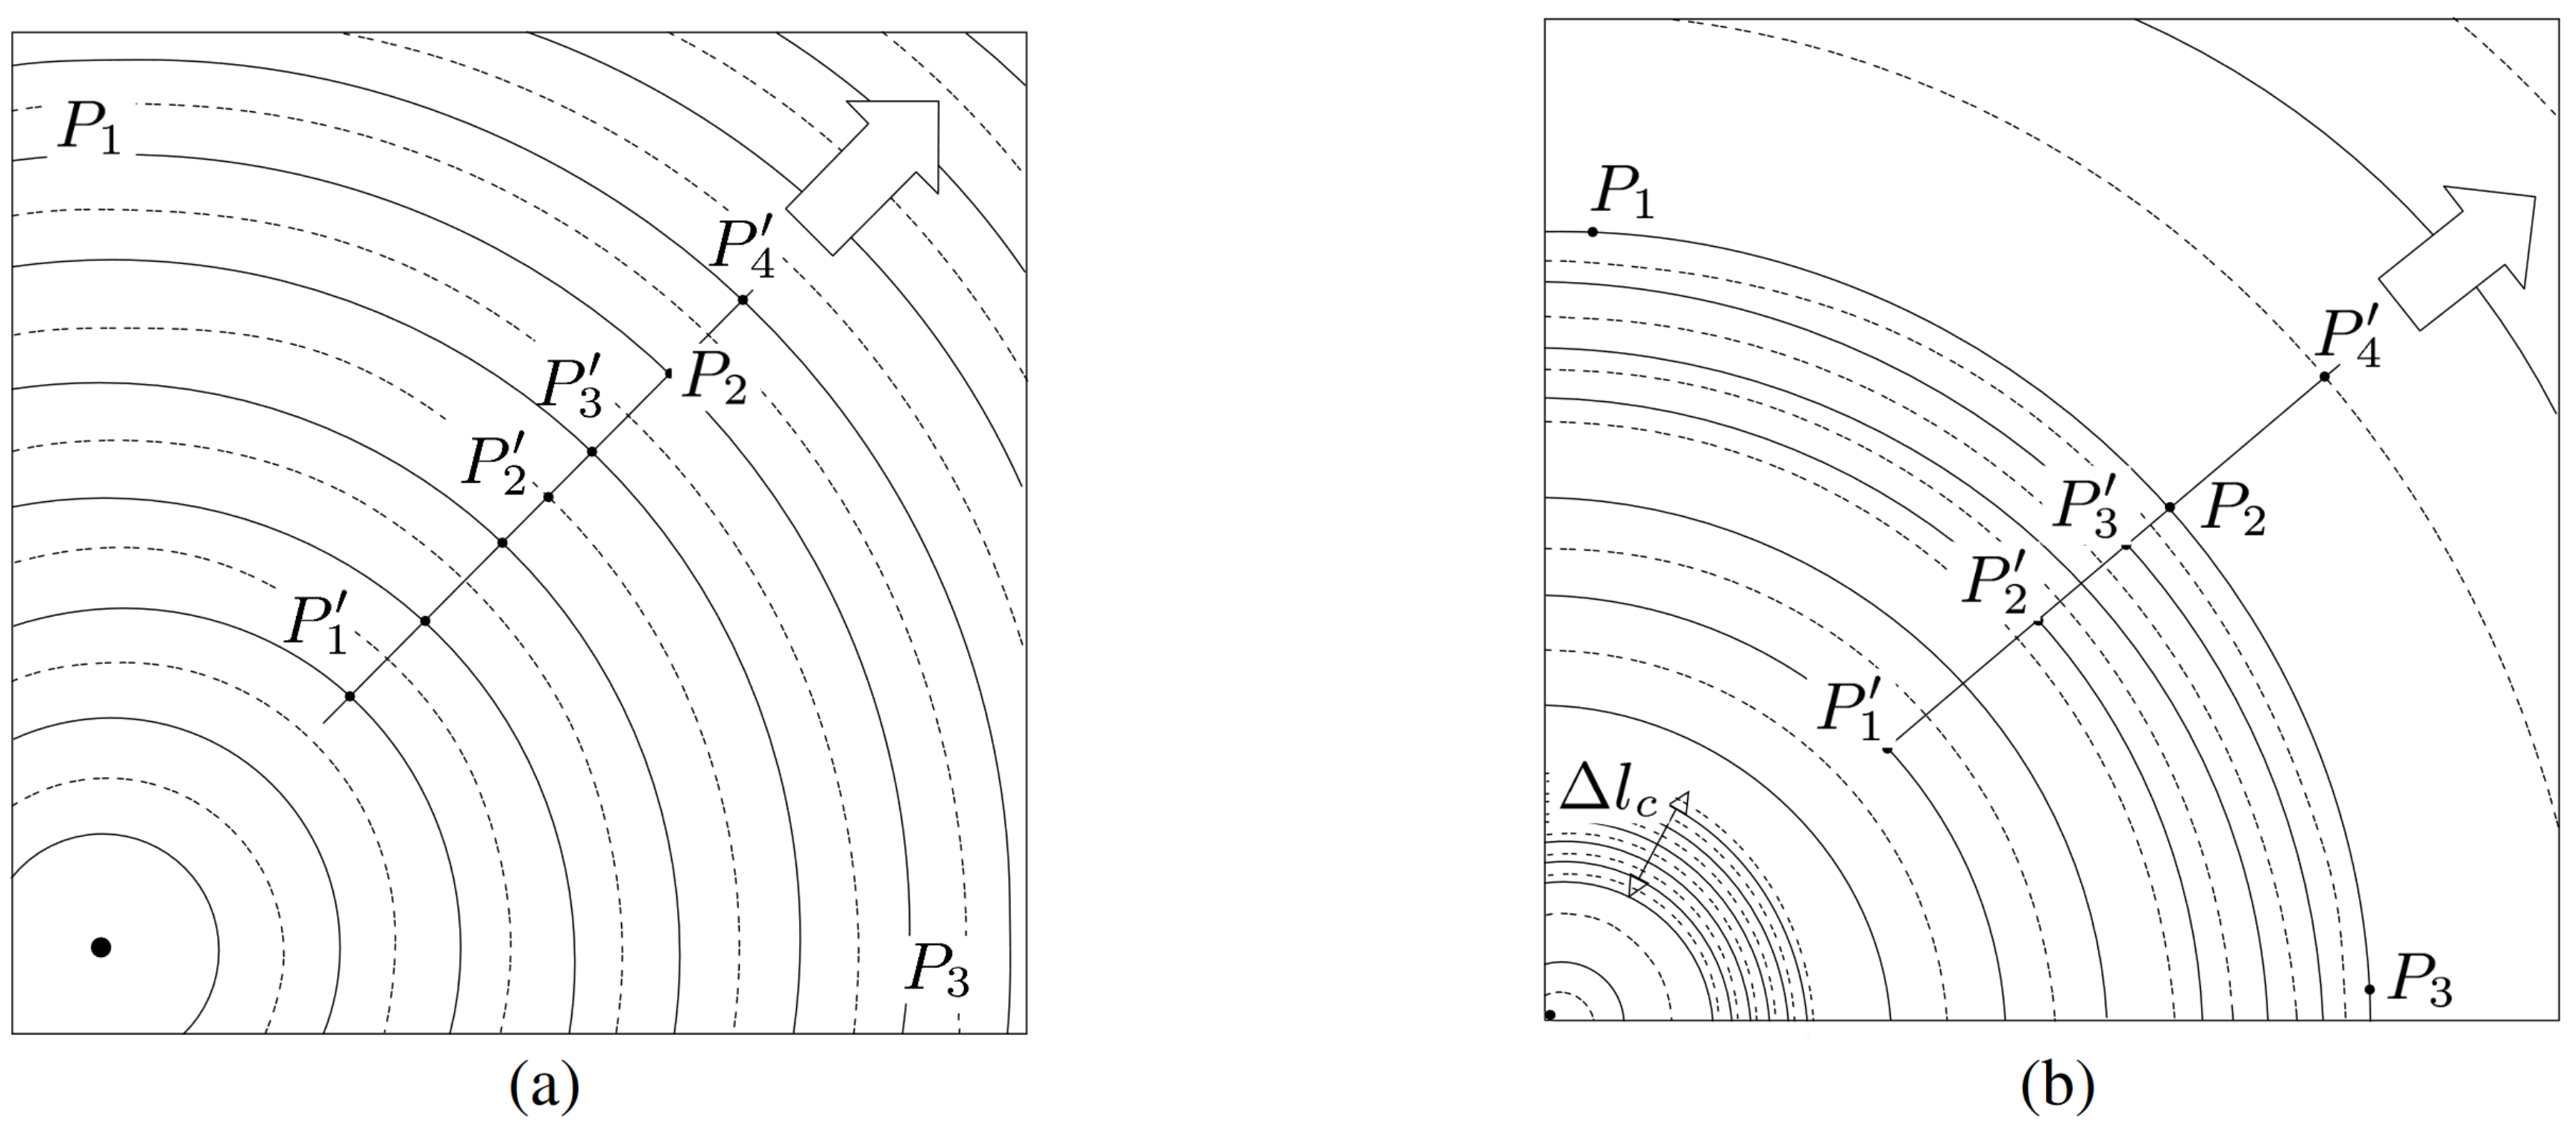
\includegraphics[width=0.8\textwidth]{images/Theorie/Hecht_9.6.png}
    \caption{Dargestellt ist eine Skizze von Wellenfronten zur Veranschaulichung von Kohärenz. In (a) ist die Welle vollständig räumlich und zeitlich kohärent. In (b) ist die Welle nur noch teilweise zeitlich kohärent, aber weiterhin räumlich kohärent. Die Kohärenzläge $\Delta l_c$ ist eingezeichnet. Abbildung entnommen aus \cite{hechtOptik2018}.}
    \label{fig:skizze kohärenz}
\end{figure}
\autoref{fig:skizze kohärenz} (a) zeigt eine vollständig kohärente Welle. Die Phasenbeziehung zwischen Punkten in Ausbreitungsrichtung ist vollkommen deterministisch, die Welle ist monochromatisch und damit zeitlich, oder longitudinal kohärent. 
Auch in transversaler Richtung (vergleiche Punkte $P_1$-$P_3$) entlang einer Wellenfront ist die Phasenbeziehung für jeden Zeitpukt identisch. 
Die Welle ist räumlich oder transversal kohärent. 
Räumliche Kohärenz liegt auch in \autoref{fig:skizze kohärenz} (b) vor. 
Allerdings ist erkennbar, dass die Welle in longitudinaler Richutung nicht für alle Distanzen eine feste Phasenbeziehung hat. 
So ist die Frequenz in $P_1'$ z.B. niedriger, als die in $P_3'$. 
Allerdings existieren trotzdem Bereiche, in welchen die Phase sich deterministisch verändert. 
Die kürzeste Länge für die dies gilt, ist die Kohärenzlänge $\Delta l_c$, die über die Ausbreitungsgeschwindigkeit $c$ mit der sog. Kohärenzzeit $\Delta l_c = c\tau_c$ zusammenhängt. 
Die Kohärenzzeit ist damit jene Zeit, für welche die Phase einer Welle vorhersehbar ist. 
Damit haben vollständig zeitlich kohärente Quellen eine unendlich lange, teilweise kohärente Quellen eine endliche Kohärenzzeit und für inkohärente Quellen gilt $\tau_c =0$. 

Die obige Abbildung motiviert bereits, dass die Kohärenzzeit ein Maß für die spektrale Breite des Lichts $\Delta \omega$ darstellt. 
Es gilt \cite{foxQuantumOpticsIntroduction2006}:
\begin{equation}
    \tau_c  \approx \frac{1}{\Delta \omega}
    \label{eq:tau(delta nu)}
\end{equation}
Da Kohärenz eine Korrelation in den Feldamplituden beschreibt, lässt sich diese Eigenschaft des Lichtes mathematisch auch mit der sog. Korrelationsfuntion erster Ordnung beschreiben. 
Diese lautet \cite{foellmiIntensityInterferometrySecondorder2009}:
\begin{equation}
    g^{(1)}(\mathbf{r_1}, t_1, \mathbf{r_2}, t_2) = \frac{\left<E^*(\mathbf{r_1}, t_1)E(\mathbf{r_2}, t_2)\right>}{\left[\left<E^*(\mathbf{r_1}, t_1)^2\right> \left<E(\mathbf{r_2}, t_2)^2\right>\right]^{1/2}}
    \label{eq:g1(r1,t1,r2,t2)}
\end{equation}
Hierbei bezeichnet $E(\mathbf{r_i},t_i)$ die komplexe Feldamplitude am Beobachtungsort $\mathbf{r_i}$ und zur Zeit $t_i$ und $\left<\dots\right>$ den Zeitmittelwert über viele Schwingungsperioden. 
\todo{Es geht glaube ich weiger um die Ausdehnung als um die Distanz zur quelle. Finde cite für rho, die erklärt das bestimt}
Unter der (für Quellen mit geringer Ausdehnung gerichtfertigten) Annahme, dass die Zeitmittelwerte der Intensitäten an den beiden Orten $\mathbf{r_1}$ und $\mathbf{r_2}$ identisch sind und der Annahme, dass die Intensität zeitlich konstant ist ($\left<I(t_1)\right>=\left<I(t_2)\right>=I$) lässt sich die Funktion weiter umschreiben. 
Weiterhin sind häufig nur Differenzen in der Zeit und im Ort relevant, anstatt absolute Orten und Zeiten zu betrachten, was folgende Variablensubstitution nahelegt: $\tau = t_2 -t_1$ und $\bm{\rho} = \mathbf{r_2} - \mathbf{r_1}$. 
Damit folgt:
\todo{citation}
\begin{equation}
    g^{(1)}(\mathbf{r}, \bm{\rho}, t, \tau) = \frac{\left<E^*(\mathbf{r}, t)E(\mathbf{r}+\bm{\rho}, t+\tau)\right>}{I}
    \label{eq:g1(r1,r2,tau)}
\end{equation}
Häufig wird zudem nur die Korrelation zweier Punkte am selben Ort, d.h. $\bm{\rho}=0$ oder zu selben Zeit, d.h. $\tau=0$, betrachtet. 
Ist dies der Fall vereinfacht sich \autoref{eq:g1(r1,r2,tau)} zur zeitlichen bzw. räumlichen Korrelationsfunktionen $g^{(1)}(\tau)$, bzw. $g^{(1)}(\bm{\rho})$.


\subsection{Michelson Sterninterferometer}
\label{ssec:Michelson Sterninterferometer}
Eine Methode die räumliche Korrelationsfunktion erster Ordnung zu messen ist das Michelson Sterninterferometer, welches schematisch in \autoref{fig:Michelson Sterninterferometer} dargestellt ist. 
\begin{figure}[htbp]
    \centering
    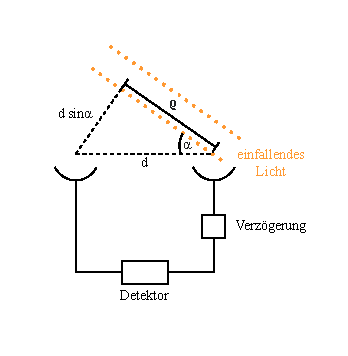
\includegraphics[width=0.5\textwidth]{images/Theorie/Michelson_Interferometer.pdf}
    \caption{Abgebildet ist eine Skizze des Michelson Sterninterferometers zur Bestimmung von Sternendurchmessern. Zwei durch die Distanz $d$ getrennte Spiegel lenken das Sternenlicht zusammen, es kommt zur Interferenz, die mit einem Detektor beobachtbar ist. Dafür wird der geometrische Streckenunterschied $d\sin\alpha$ durch Verzögerungen kompensiert, um dieselbe Wellenfront zu vergleichen. Abbildung inspiriert von \cite[Fig. 1]{foellmiIntensityInterferometrySecondorder2009}.}
    \label{fig:Michelson Sterninterferometer}
\end{figure}
Der historische Grund für die Entwicklung von Interferometern zur Beobachtung von Sternen liegt im Ziel, immer bessere Winkelauflösungen erreichen zu wollen. 
Während für die Winkelauflösung gewöhnlicher Teleskope $\theta \propto \frac{\lambda}{D}$ gilt, gilt für Interferometer $\theta \propto \frac{\lambda}{d}$. 
\todo{citation}
Hierbei ist $\lambda$ die Wellenlänge, $D$ der Durchmesser der Teleskopöffnung (je nach Bauart der Hauptspiegel oder die Linse) und $d$ der Abstand zwischen Teleskopen die ein Interferometer bilden. 
Da es technisch schwierig ist, beliebig große Spiegel- bzw. Linsendurchmesser anzufertigen, sind optische Teleskope auf eine vergleichsweise geringe Auflösung im Bereich von einigen Bogensekunden limitiert. 
So erreicht z.B. das \emph{Gran Telescopio Canarias} (GTC) eine Auflösung von etwa 12\,masec bei $\lambda=500\,\mathrm{nm}$ und $D=10,4\,\mathrm{m}$ \cite{GranTelescopioCANARIAS}. 
Obwohl es Bestrebungen gibt immer größere Einzelspiegelteleskope zu bauen, besteht eine weitere, technisch einfachere Herangehensweise darin, das Licht vieler kleiner Teleskope zu kombinieren. 
Dies ist die Grundidee des Michelson Sterninterferometers, welches aus zwei Teleskopen besteht, die durch eine Distanz $d$ voneinander getrennt sind. 
Diese bündeln das Licht, welches anschließend zusammengeführt und zur Interferenz gebracht wird. 
Durch dieses Vorgehen lassen sich deutlich bessere Winkelauflösungen bewerkstelligen. 
So erreicht z.B. das Ende der 1980er gebaute \emph{Sydney University Stellar Interferometer} (SUSI) Auflösungen von $70\,\mathrm{\mu asec}$ bei $\lambda=450\,\mathrm{nm}$ und $d=640\,\mathrm{m}$ \cite{davisSydneyUniversityStellar1999}. 
Ein Nachteil des Interferometers ist allerdings eine erniedrigte Sensitivität im Vergleich zu gewöhlichen Teleskopen. 
Da die Lichtsammelfläche zweier kleiner Teleskope für gewöhnlich kleiner ist als die eines großen Einzelspiegels, wird weniger Licht gesammelt, was interfermoterische Verfahren auf besonders helle Sterne limitiert \cite{foxQuantumOpticsIntroduction2006}. 
Weiterhin wird statt einem zweidimensionalen Bild lediglich eine eindimensionale Größe, nämlich der Winkeldurchmesser des Sternes bestimmt. 
Durch den Zusammenschluss vieler Teleskope, kann allerdings trotzdem auf die zweidimensionale Helligkeitsverteilung rückgeschlossen werden. 
Weiterführendes findet man unter dem  Stichpunkt \glqq Aperture Synthesis \grqq z.B. in \cite[Kap. 10]{burkeIntroductionRadioAstronomy2019}. \\

Beobachtungsziel des Inteferometers ist ein Stern, also eine ausgedehnte, thermische Lichtquelle. 
Thermisches Licht ist zwar grundsätzlich nicht kohärent, aber ein Gedankenexperiment zeigt auf, dass durch das Samplen des Lichts an zwei weit vom Stern entfernten Orten trotzdem teilweise Kohärenz vorliegen kann. 
Man kann sich eine ausgedehnte Lichtquelle als die Superposition vieler infinitesimal kleiner Punktqullen vorstellen. 
Jede dieser Punktquellen hat für sich genommen keine Winkelausdehnung und bildet damit im Fernfeld eine vollständig räumlich kohärente ebene Welle. 
\todo{verstehen. Sicher das die Punktquellen kohärent sind??? Finde Quelle wo das steht}
Die Überlagerung der Punktquellen bedeutet nun im Fernfeld eine Überlagerung vieler für sich genommen räumlich kohärenten aber untereinander inkohärenten ebenen Wellen. 
Da in jedem Teleskop des Interferometers eine Vielzahl dieser ebenen Wellen detektiert wird, verbleibt eine gewisse Ähnlichkeit zwischen den detektierten Feldern - Die beiden Felder sind teilweise korreliert. 
Dies ist in \autoref{fig:räumliche kohärenz einer ausgedehnten quelle} dargestellt. 
\begin{figure}[htbp]
    \centering
    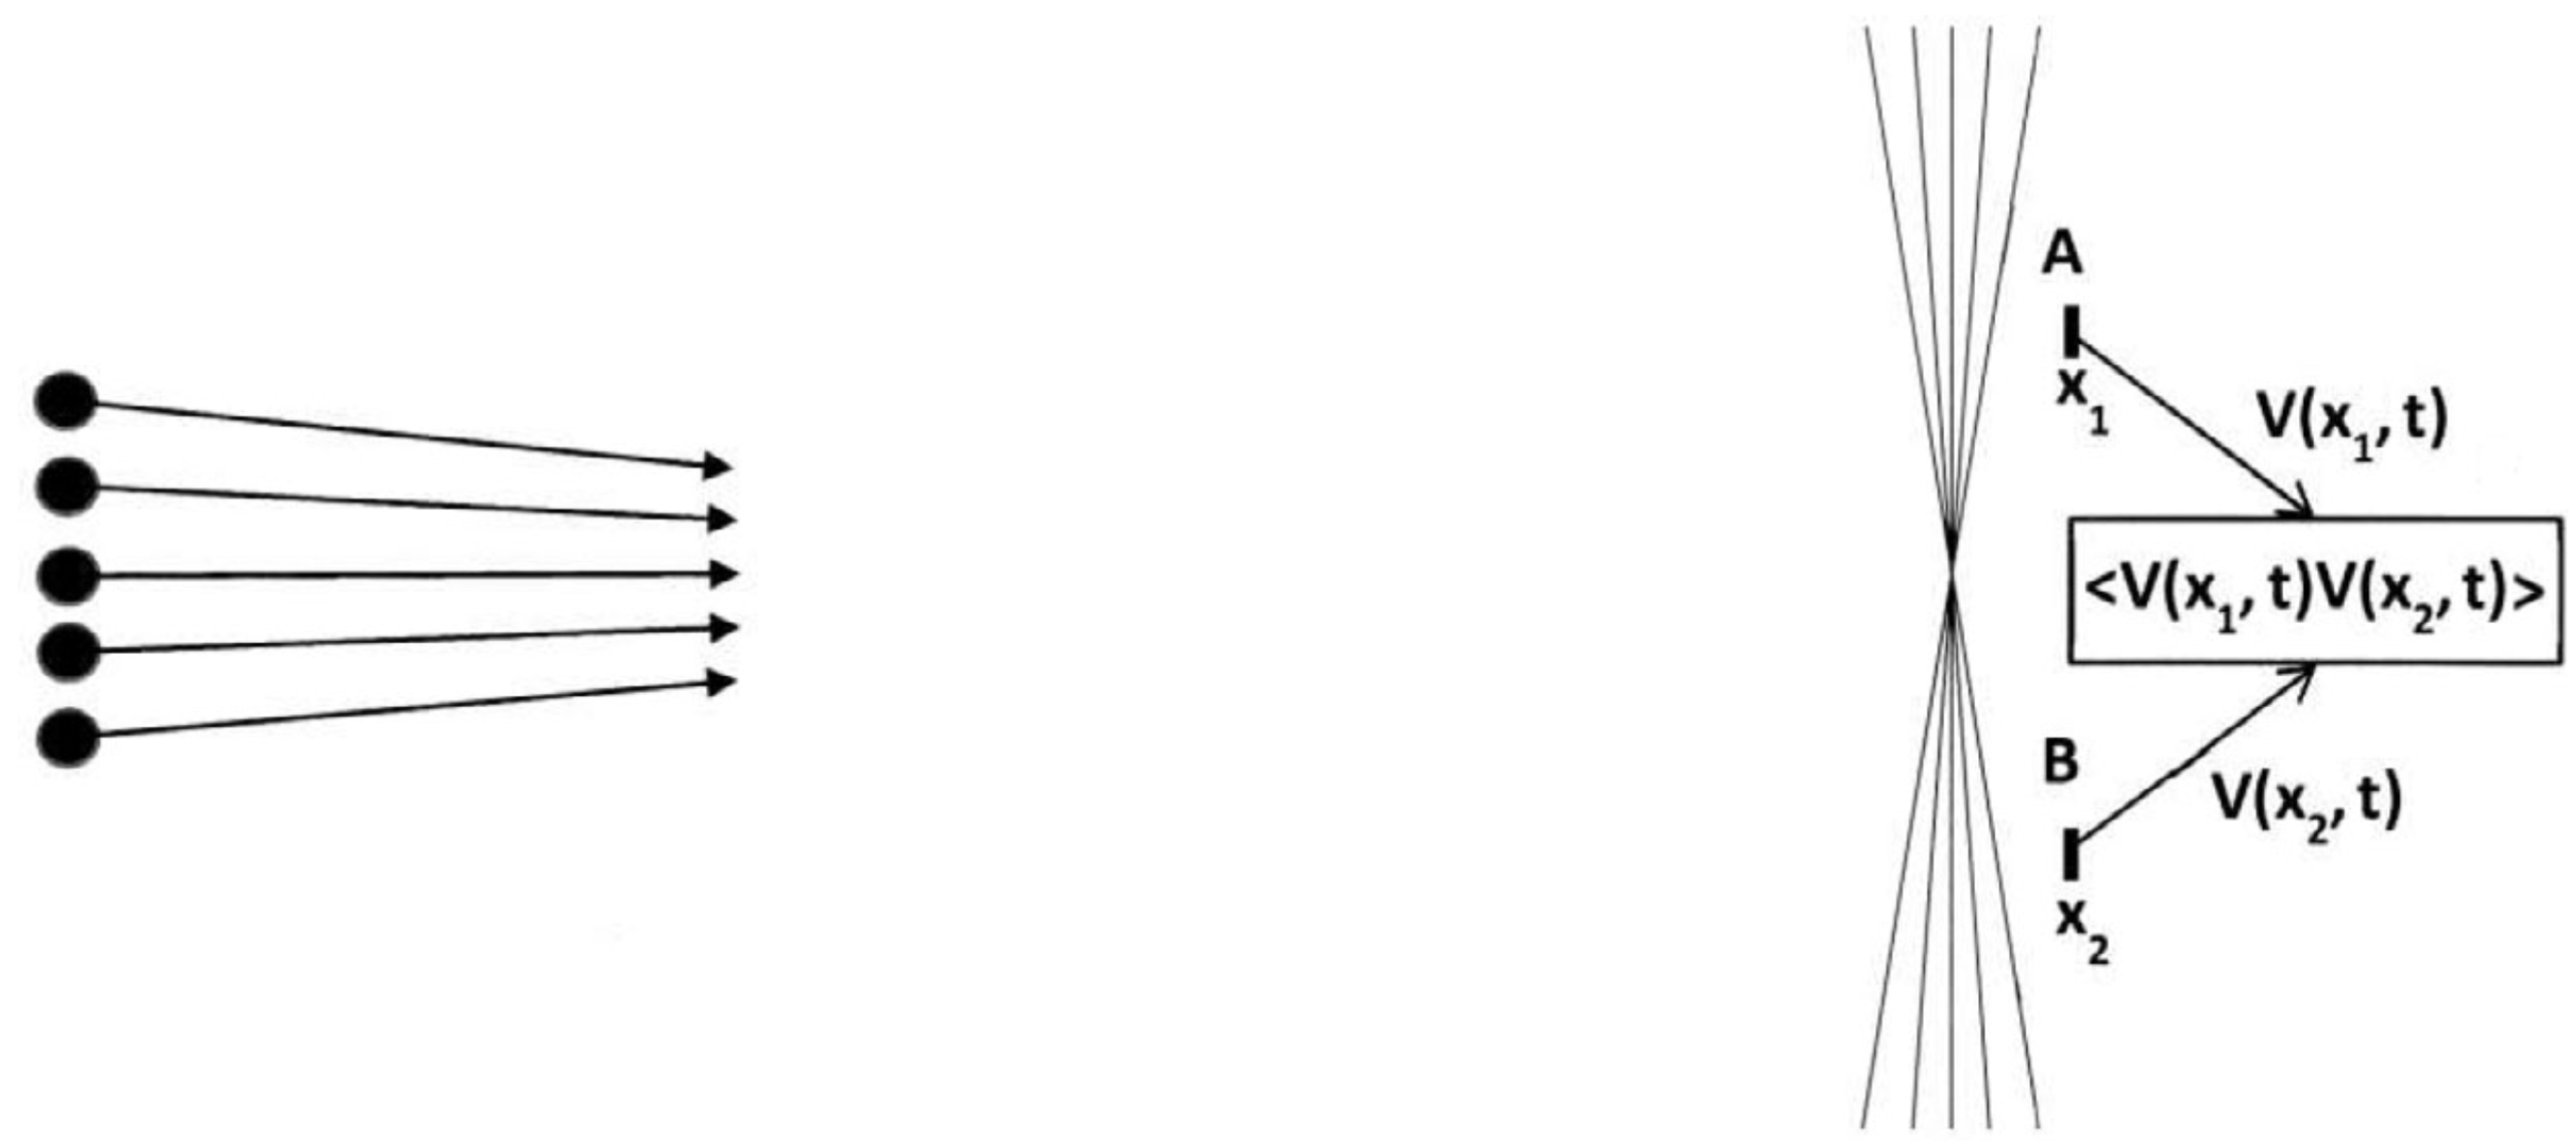
\includegraphics[width=0.8\textwidth]{images/Theorie/Burke_9.25.png}
    \caption{Abgebildet ist eine Skizze die veranschaulicht, wie eine ausgedehnte inkohärente Quelle bei Teleskopseparationen $d\lesssim\Delta l_c$ trotzdem teilweise korreliertes Licht aufweist. Links ist eine Quelle schematisch in viele kohärente Punktquellen zerlegt, die ebene Wellen emittieren. In beiden Detektoren werden jeweils alle ebenen Wellen detektiert, allerdings kommen diese aufgrund der Geometrie zu leicht verschiedenen Zeiten an. Es ist deutlich, dass die Lichtfelder für steigende $d$ immer verschiedener werden (die Kohärenz sinkt), während sie für $d=0$ vollkommen identisch und somit kohärent wären. Die Abbildung ist \cite[Fig. 9.25]{burkeIntroductionRadioAstronomy2019} entnommen.}
    \label{fig:räumliche kohärenz einer ausgedehnten quelle}
\end{figure}
\todo{Warum muss die Quelle klein sein?}
Diese Korrelation ist maximal für eine Teleskopseparation von $d=0$, da in diesem Fall in beiden Teleskopen exakt dasselbe Licht gemessen wird. 
Wird $d$ nun immer weiter erhöht, verringert sich die Korrelation zwischen den Feldern immer weiter, die Lichtfelder bestehen aus immer verschiedeneren ebenen Wellen und sind sich weniger ähnlich. 
Ab einer Separation $d\gtrsim\Delta l_c$ sind die Lichtfelder nicht mehr korreliert und $g^{(1)}$ fällt auf Null ab. 
Für spektral breites Licht (wie es für das thermische Licht von Sternen üblich ist) ist die erwartete maximale Teleskopseparation sehr klein, vgl. \autoref{eq:tau(delta nu)}. 
Daher wird häufig auf entsprechend enge Lichtfilter zurückgegriffen, die die spektrale Breite des Lichts heruntersetzen um die Kohärenzlänge zu erhöhen. \\


Messgröße des Michelson Sterninterferometers ist im einfachsten Fall der Interferenzkontrast, definiert als \cite{foellmiIntensityInterferometrySecondorder2009}
\begin{equation}
    K = \frac{I_{max}-I_{min}}{I_{max}+I_{min}}=\left|g^{(1)}(\mathbf{r}, \bm{\rho}, t, \tau)\right|
\end{equation} 
Hierbei sind $I_{max}$, bzw. $I_{min}$ die Intensitätsmaxima, bzw. -minima der gemessenen Intensität auf dem Schirm. 
$\tau$ ist hierbei die Zeitdifferenz zwischen den beiden Feldern, die durch die Strecke $d\cdot\sin \alpha$ in \autoref{fig:Michelson Sterninterferometer} entsteht und $\bm{\rho}$ der effektive Abstandsvektor zwischen den Teleskopen. 
Der effektive Teleskopabstand entspricht der Projektion des Teleskopabstandes $d$ in die Beobachtungsebene, die i.A. nicht parallel zu $d$ liegt. 
Durch komplexere Methoden lässt sich neben der Amplitude auch die Phase der komplexen Funktion $g^{(1)}(\mathbf{r}, \bm{\rho}, t, \tau)$ messen, vgl. dazu \cite[Kap. 4.3]{mandelOpticalCoherenceQuantum1995}. \\
Die Messung eines Sternendurchmessers lässt sich nun wie folgt bewerkstelligen. 
Im Interferometer wird die Weglängendifferenz $d \sin \alpha$ durch die Wahl einer passenden Verzögerung kompensiert, sodass die Welle zwar an zwei verschiedenen Orten, aber effektiv zu ein und derselben Zeit gesampelt wird. 
$\tau=0$ und die Welle ist zeitlich kohärent \cite{foellmiIntensityInterferometrySecondorder2009}. 
Durch Messung des Interferenzkontrastes für verschiedene effektive Spiegelseparationen $\rho=|\bm{\rho}|$, lässt sich die räumliche Korrelationsfunktion erster Ordnung messen. 
Über das van-Cittert-Zernike Theorem lässt sich aus der gemessenen räumlichen Korrelationsfunktion nun über eine Fouriertransformation auf die Intensitätsverteilung der Quelle zurückschließen:
\begin{equation}
    \dots
\end{equation}
\todo{vZZ theorem}

Der Vollständigkeit halber soll hier auch auf die Rolle der zeitlichen Korrelation $g^{(1)}(\tau)$ eingegangen werden. 
Diese stellt zwar bei interferometrischen Beobachtungen selten die primäre Observable dar, enthält aber trotzdem Informationen über die Quelle. 
Während die räumliche Korrelationsfunktion erster Ordnung mit dem Intensitätsprofil der Quelle zusammenhängt, gilt für $g^{(2)}(\tau)$ das Wiener-Khintchine Theorem \cite{lasseguesFieldIntensityCorrelations2022}:
\begin{equation}
    S(\omega) =  \int g^{(1)}(\tau) e^{i\omega\tau} d\tau
\end{equation}
Das Spektrum der Quelle $S(\omega)$ ist die Fouriertransformierte der zeitlichen Korrelationsfunktion erster Ordnung. \\
Auch wenn wie erwähnt $g^{(1)}(\tau)$ häufig nicht die primäre Observable ist, soll hier noch einmal explizit erwähnt werden, dass für eine interferometrische Beobachtung nie \emph{nur} die räumliche Kohärenz der Quelle ausschlaggebend ist. 
Räumlich Kohärenz herrscht wie bereits erwähnt nur innerhalb eines Kohärenzvolumens $(\Delta l_c) ^3$. 
Für die Messung der räumlichen Kohärenz ist also stets zu beachten, dass das Licht durch optische Filter spektral so verengt werden muss, dass Kohärenzlängen erzeugt werden, die eine Beobachtung bei ausreichend großen Teleskopseparationen erlauben. \\

Ein Nachteil des Michelson Sterninterferometers ist die schwierig herzustellende Stabilität im Teleskop. 
Da die Wellen direkt miteinander interferieren, muss der Weg des Lichts auf einen Bruchteil einer Wellenlänge stabilisiert werden, um Phasenstabilität sicherzustellen. 
Dies wird insbesondere schwieriger, je größer die Spiegelabstände werden, was das Herstellen großer Winkelauflösungen erschwert. 
Weiterhin induzieren atmosphärische Variabilitäten schwer vorherzusagende Phasendifferenzen zwischen den beiden Teleskopen, die das Interferenzenmuster beeinflussen \cite[Kap. 2]{brownIntensityInterferometerIts1974}. 
Durch dieses sogenannte \glqq Seeing\grqq\;und die Notwendigkeit eines mechanisch sehr präzisen und stabilen Aufbaus, sind Michelson Sterninterferometer in ihrer Größe limitiert. 
Um beide Probleme zu umgehen, haben Hanbury Brown und Twiss ein modifiziertes System entwickelt - das Intensitäteninterferometer.

\subsection{Intensitäteninterferometrie}
\label{ssec:Intensitäteninterferometrie}
Im Gegensatz zum Michelson Sterninterferometer, in dem die Amplituden der Lichtwellen direkt zur Interferenz gebracht werden, werden im von Hanbury Brown und Twiss erstmals 1955 im Labor durchgeführten Experiment \cite{brownCorrelationPhotonsTwo1956} die bereits gemessenen Intensitäten miteinander korreliert. 
Bereits in den 1960ern und 70ern entwickeln Brown und Twiss anschließend das erste Intensitäteninterferometer, das \emph{Narrabi Stellar Intensity Interferometer} und bestimmen die Winkeldurchmesser von 32 Sternen \cite[Kap. 1]{brownIntensityInterferometerIts1974}. \\
Dies war nur möglich, aufgrund des vergleichsweise einfachen Aufbaus. 
An beiden Teleskopen wird unabhängig der Photonenstrom, z.B. mittels Photomultipliern, digitalisiert und anschließend elektronisch korreliert. 
Vor- und Nachteil dieser Vorgehensweise ist die Insensitivität gegenüber Phasenunterschieden zwischen dem eintreffenden Licht an beiden Teleskopen. 
Einerseits geht durch die Messung Information (über die Phase) verloren, andererseits wird der Aufbau einfacher, da weder Phasenstabilität zwischen Teleskopen, noch atmosphärisches Seeing einen Einfluss auf das korrelierte Signal haben.
Dieses Vorgehen ermöglicht im Prinzip beliebig lange Separationen und damit beliebig gute Winkelauflösungen. 
Vorraussetzung dafür ist allerdings, die Distanz zwischen Telskopen im Vergleich zur Kohärenzlänge genau zu kennen \cite{foellmiIntensityInterferometrySecondorder2009}. 
So werden durch die \emph{Event Horizon Collaboration} z.B. mittels Intensitäteninterferometrie im Radiowellenbereich Teleskopseperationen vom Durchmesser der Erde und damit Auflösungen von etwa 25\,$\mu$asec erreicht (s. z.B. \cite{collaborationFirstSagittariusEvent2022}). \\

Eine schematische Darstellung des Intensitäteninterferometers ist in \autoref{fig:Intensitäteninterferometer} dargestellt. 
\begin{figure}[htbp]
    \centering
    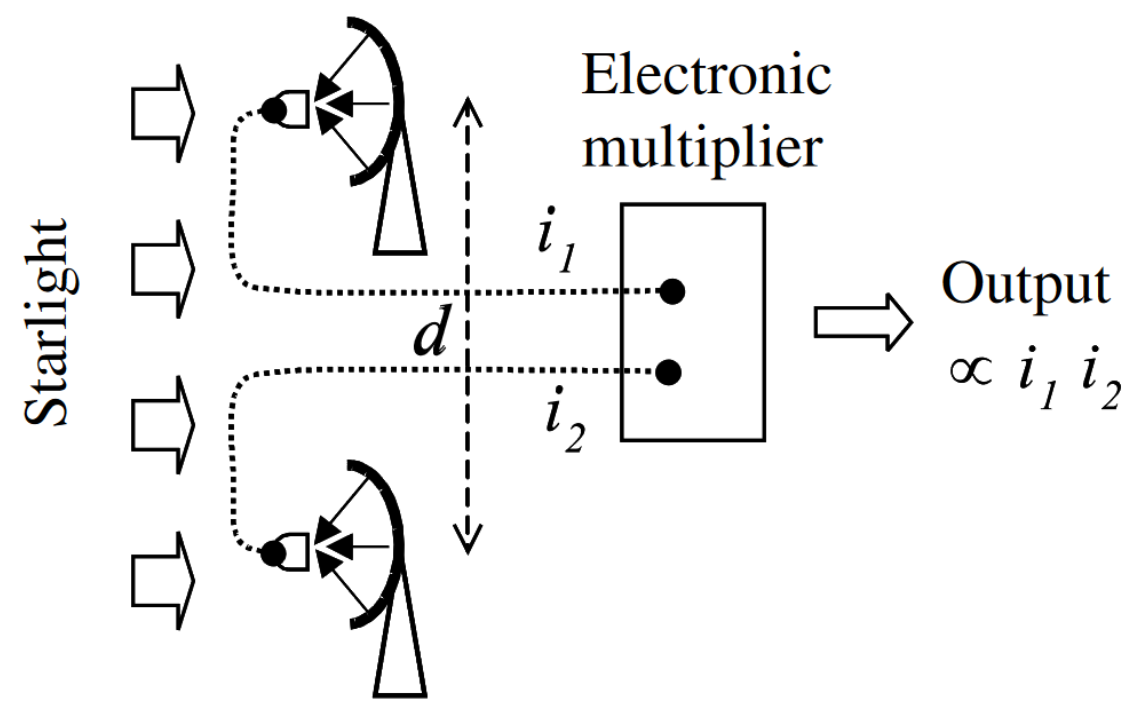
\includegraphics[width=0.5\textwidth]{images/Theorie/Fox_6.1b.png}
    \caption{Eine Skizze des Intensitäteninterferometers ist abgebildet. Das gesammelte Licht wird direkt detektiert und das zu den Intensitäten proportionale Signal elektronisch kombiniert. Entnommen aus \cite[Fig. 6.1(b)]{foxQuantumOpticsIntroduction2006}.}
    \label{fig:Intensitäteninterferometer}
\end{figure}

Zur Beschreibung der Korrelation von Intensitäten ist eine Erweiterung der bisher genannten Theorie nötig. 
Es bietet sich an, eine Korrelationsfunktion zweiter Ordnung einzuführen:
\todo{chekc eq, finde zitate für die Schritte (Foellmi macht das so n bisschen)}
\begin{equation}
    g^{(2)}(\mathbf{r_1}, t_1, \mathbf{r_2}, t_2) = \frac{\left<E^*(\mathbf{r_1}, t_1)E^*(\mathbf{r_2}, t_2)E(\mathbf{r_2}, t_2)E(\mathbf{r_1}, t_1)\right>}{\left<E^*(\mathbf{r_1}, t_1)E(\mathbf{r_1}, t_1)\right> \left<E^*(\mathbf{r_2}, t_2)E(\mathbf{r_2}, t_2)\right> }
\end{equation}
Dies lässt sich durch $\bm{\rho} = \mathbf{r_2} - \mathbf{r_1}$ und $\tau = t_2 - t_1$ erneut in relative räumliche und zeitliche Distanzen umformulieren. Weiterhin kann erneut verwendet werden, dass die mittlere Intensität an $\mathbf{r}$ etwa gleich der an $\mathbf{r} +\bm{\rho}$ ist, da die  Quelle weit entfernt ist und dass die mittlere Intensität zeitlich konstant ist, sodass gilt $\left<I(t)\right> = \left<I(t+\tau)\right>$. Mit der Notation $I=\left<I(t)\right>$ erhält man:
\begin{equation}
    g^{(2)}(\mathbf{r}, \bm{\rho}, t, \tau) = \frac{\left<E^*(\mathbf{r}, t)E^*(\mathbf{r+\rho}, t+\tau)E(\mathbf{r+\rho}, t+\tau)E(\mathbf{r}, t)\right>}{I^2}
\end{equation}
Unter der Annahme von thermischem, bzw. chaotischem Licht, in dem die Phasen der individuellen emittierten Lichtquanten zufällig verteilt sind, folgt:
\begin{equation}
    g^{(2)}(\mathbf{r}, \bm{\rho}, t, \tau) =  \frac{\left<I(\mathbf{r}, t) I(\mathbf{r}+\bm{\rho}, t+\tau)\right>}{I^2}
\end{equation}
Durch das Interferometer kann nun (analog zu $g^{(1)}(\bm{\rho})$ beim Michelson Sterninterferometer) $g^{(2)}(\bm{\rho})$ gemessen werden. 
Um nun trotzdem auf die Quellengeometrie schließen zu können, wird ein Zusammenhang zwischen $g^{(1)}$ und $g^{(2)}$, die sog. Siegert Relation genutzt \cite{lasseguesFieldIntensityCorrelations2022}:
\begin{equation}
    g^{(2)}(\tau) = 1+ \left|g^{(1)}(\tau)\right|^2
\end{equation}
Diese gilt nur für chaotisches und thermisches Licht. 
Unter chaotischem Licht versteht man Licht, dessen Quanten aufgrund von Stößen unter emittierenden Gasmolekülen und der Eigenbewegung dieser mit zufälliger Phase emittiert werden. 
Es weist ähnlich wie thermisches Licht, welches Schwarzkörperstrahlung entspricht, Intensitätsschwankungen auf der  Zeitskala einer Kohärenzzeit auf. 
Ein Beispiel für thermisches Licht ist die Emission eines Sterns und ein Beispiel für chaotisches Licht das Licht einer Gasentladungslampe \cite{foxQuantumOpticsIntroduction2006}. 
Über eine Messung von $g^{(2)}$ mit dem Intensitäteninterferometer kann so mit der Siegert Relation auf $g^{(1)}$ und anschließend mit dem van Cittert-Zernike Theorem auf die Quellengeometrie geschlossen werden. 
In \autoref{fig:g1(rho),g2(rho) für versch Lochblenden} ist vergleichend der Verlauf von $g^{(1)}(\rho)$ und $g^{(2)}(\rho)$ dargestellt. 
Hierbei wird als Lichtquelle eine uniform ausgeleuchtete Lochblende des Durchmessers $d$ im Abstand $x$ angenommen. 
Dies entspricht im einfachsten Sternmodell einer uniform leuchtenden Scheibe einem Stern mit Winkeldurchmesser $\Delta \theta = \frac{d}{x}$. 
Für dieses Modell gilt nach \cite[Kap. 4.1]{brownIntensityInterferometerIts1974}:
\begin{align}
    \left| g^{(1)}(\rho)\right| &= \frac{2J_1\left(\frac{\pi\rho\Delta\theta}{\lambda_0}\right)}{\frac{\pi\rho\Delta\theta}{\lambda_0}}\quad\quad\quad \Rightarrow & g^{(2)}(\rho) &= 1 + \left[\frac{2J_1\left(\frac{\pi\rho\Delta\theta}{\lambda_0}\right)}{\frac{\pi\rho\Delta\theta}{\lambda_0}}\right]^2
\end{align}
Hierbei ist $J_1$ die Besselfunktion erster Ordnung und $\lambda_0$ die zentrale Wellenlänge, gegeben durch den verwendeten Filter. 
Für Werte von $x=1,75\,\mathrm{m}$ und $\lambda_0=465\,\mathrm{nm}$ ergeben sich die in \autoref{fig:g1(rho),g2(rho) für versch Lochblenden} gezeigten Verläufe. 
\begin{figure}[htbp]
    \centering
    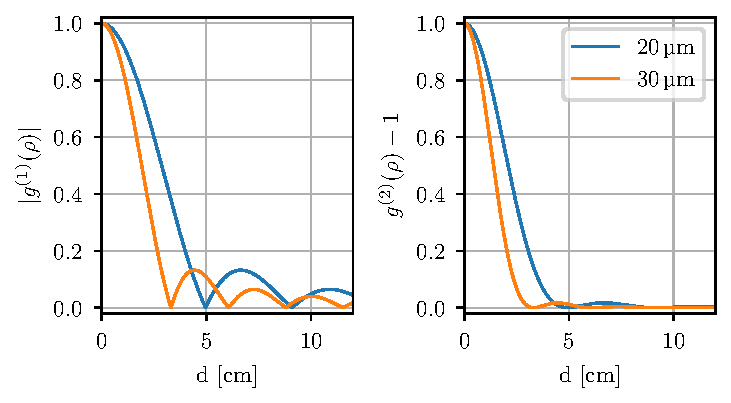
\includegraphics{images/Theorie/g1_g2_rho.pdf}
    \caption{Gezeigt sind die Verläufe von $g^{(1)}(\rho)$ und $g^{(2)}(\rho)$ für zwei Lochblende mit Durchmesser $20\,\mathrm{\mu m}$ und $10\,\mathrm{\mu m}$. Für beide Lochblenden ist $x=1,75\,\mathrm{m}$ und $\lambda_0=465\,\mathrm{nm}$.}
    \label{fig:g1(rho),g2(rho) für versch Lochblenden}
\end{figure}
Durch samplen der Funktion $g^{(2)}(\rho)$ kann die erste Nullstelle bestimmt werden, die für das genannte Modell bei 
\begin{equation}
    \rho=1,22\frac{\lambda_0}{\Delta\theta} 
    \label{eq:erste nulstelle von g2(rho) für lochblende}
\end{equation}
liegt \cite[Kap. 4.1]{brownIntensityInterferometerIts1974}. 
Aus dieser kann dann der Winkeldurchmesser berechent werden. \\


Um $g^{(2)}(\rho)$ für verschiedene effektive Teleskopseparationen zu samplen, wird für jede Distanz $\rho=|\bm{\rho}|$ die zeitliche Kohärenzfunktion zweiter Ordnung gemessen, indem die digitalisierten Intensitäten miteinander korreliert werden. 
Deswegen soll im Folgenden der erwartete Verlauf der Observablen $g^{(2)}(\tau)$ näher beschrieben werden. 
Anhand des Verhaltens von $g^{(2)}(0)$ lassen sich drei Phänomene unterscheiden \cite{foxQuantumOpticsIntroduction2006}. 
\begin{itemize}
    \item $g^{(2)}(0)=1$: Die Photonen treffen mit zufälligen Abständen auf den Detektor. Das Licht ist kohärent und es gilt allgemein $g^{(2)}(\tau)=1$. In guter Näherung gilt dies für Laserlicht.
    \item $g^{(2)}(0)>1$: Die Photonen erreichen die Detektoren gebündelt in sog. \emph{bunches}. Die Korrelation ist erhöht bei niedrigen Zeitdifferenzen, mit anderen Worten ist es also wahrscheinlicher ein weiteres Photon zu messen, wenn zuvor bereits eines gemessen wurde. Thermisches und chaotisches Licht zeigen bunching.
    \item $g^{(2)}(0)<1$: Die Photonen treffen in regelmäßigen Abständen auf den Detektor. Dieses Phänomen bezeichnet man als \emph{antibunching}. 
\end{itemize}
Eine Veranschaulichung der Einteilung des Lichtes ist in \autoref{fig:bunching} gezeigt. 
\begin{figure}[htbp]
    \centering
    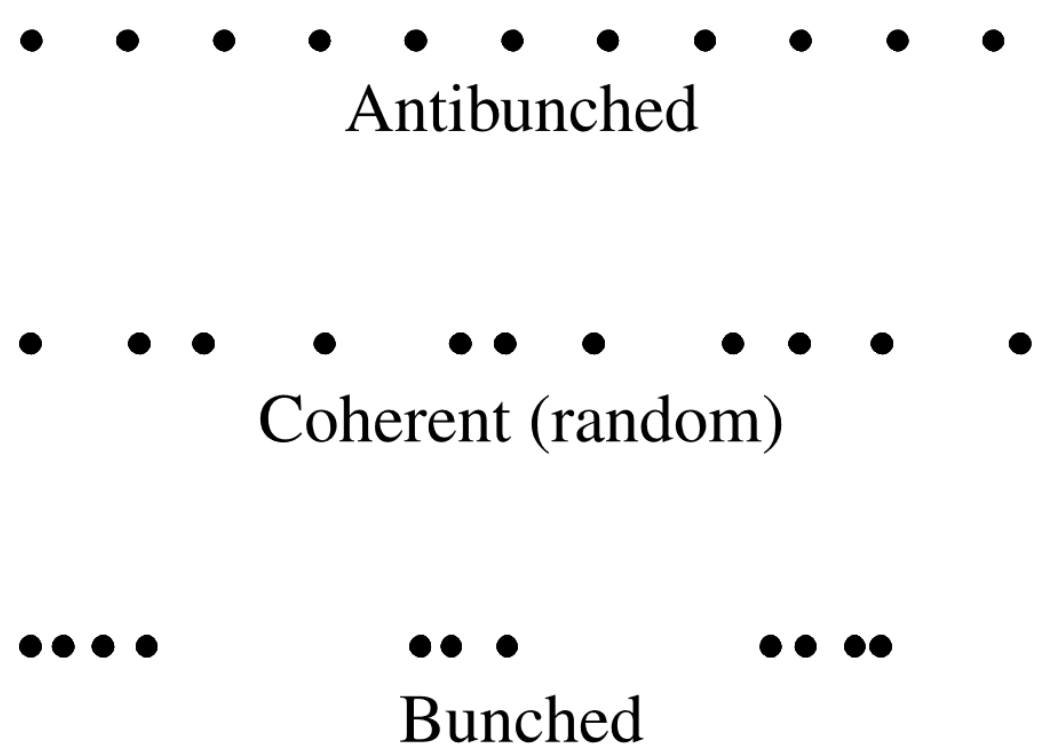
\includegraphics[width=0.4\textwidth]{images/Theorie/Fox_6.6.png}
    \caption{Anitbunching, bunching und kohärente Photonen sind schematisch dargestellt. Während die Photonenabstände bei kohärentem Licht zufällig sind, sind bei antibunching regelmäßige und bei bunching geringe Abstände wahrscheinlicher. Abbildung aus \cite[Fig. 6.6]{foxQuantumOpticsIntroduction2006}}
    \label{fig:bunching}
\end{figure}
Eine weitere geläufige Einteilung des Lichts wird aufgrund der Photonenstatistik, also der Verteilung der gemessenen Einzelphotonen in einem gewissen Zeitintervall, vorgenommen. 
Nach dieser Einteilung ist die Anzahl gemessener kohärenter Photonen poissonverteilt, während gebunchte Photonen eine breitere und antigebunchte Photonen einer schmaleren Verteilung folgen. 
Eine tiefergehende Behandlung findet sich z.B. in \cite[Kap. 5.4-5.6]{foxQuantumOpticsIntroduction2006}. \\

Durch die Siegert Relation und den bereits beschriebenen Verlauf von $g^{(1)}(\tau)$, lässt sich auf das Aussehen von $g^{(2)}(\tau)$ schließen (vgl. \cite[Kap. 6.3]{foxQuantumOpticsIntroduction2006}). 
So ist bei einem idealen Detektor $g^{(2)}(0)=2$ und fällt für $|\tau|>0$ immer weiter ab, bis sich $g^{(2)}$ nach der Kohärenzzeit, also für $\tau>\tau_c$, dem Wert 1 annähert. 
Da $g^{(2)}(\tau)$ bei chaotischen Lichtquellen wie bereits erwähnt über eine Fouriertransformation mit dem Spektrum der Quelle zusammenhängt, ergibt sich je nach verwendetem Filter ein anderer Verlauf von $g^{(2)}(\tau)$ zwischen $\tau=0$ und $\tau \gg \tau_c$. 
Der Verlauf von $g^{(1)}(\tau)$ und $g^{(2)}(\tau)$ ist in \autoref{fig:g1(tau),g2(tau) für versch Filter} für einen rechteckigen Filter mit zentraler Wellenlänge 465\,nm und Breite 10\,nm und 5 \,nm aufgezeigt. 
Für die (normalisierte) Fouriertransformation eines Rechteckpulses $rect\left(\frac{\omega}{\Delta\omega}\right)$ und damit $g^{(1)}(\tau)$ gilt:
\begin{align}
    g^{(1)}(\tau) &= sinc\left(\tau\Delta\omega\right) \quad\quad\quad \Rightarrow& g^{(2)}(\tau) &= 1+ \left[sinc\left(\tau\Delta\omega\right)\right]^2
\end{align}
\todo{citation, derzeit wikipedia}
\begin{figure}[htbp]
    \centering
    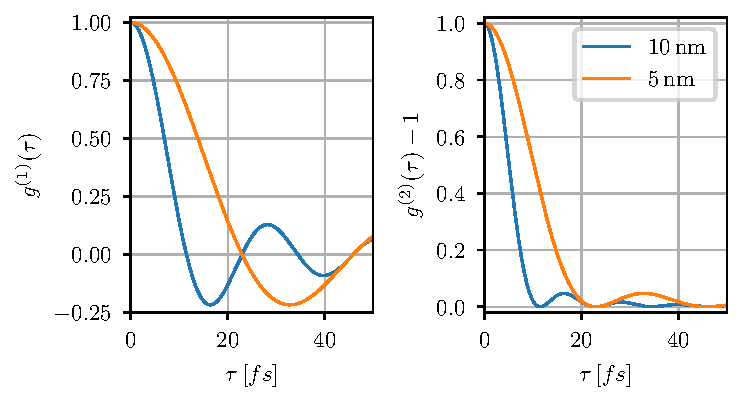
\includegraphics{images/Theorie/g1_g2_tau.pdf}
    \caption{Abgebildet ist der Theorieverlauf von $g^{(1)}(\tau)$ und $g^{(2)}(\tau)$ für einen Filter mit rechteckigem Transmissionsprofil mit Breite 10\,nm zentriert um 465\,nm.}
    \label{fig:g1(tau),g2(tau) für versch Filter}
\end{figure}
In einer realen Messung verringert die Zeitauflösung des Detektors $\tau_D$ den Wert von $g^{(2)}(0)$ zusätzlich. 
Da diese zumeist deutlich größer ist als die Kohärenzzeit, werden im zentralen Bin $\tau \in [0, \tau_D]$ neben den kohärenten Photonen auch ein Faktor $\frac{\tau_D}{\tau_c}$ mehr zufällig koinzidente Photonen gemessen. 
Dies verringert $g^{(2)}(0)$ um ebendiesen Faktor \cite[Kap. 14.7]{mandelOpticalCoherenceQuantum1995}. 
Dies verdeutlicht eine weitere Herausforderung in der angewandten Intensitäteninterferometrie. 
Da die Zeitauflösung des Detektors oft deutlich geringer ist als die Kohärenzzeit, ist das zu messende Signal sehr klein, was ein geringes Signal zu Rausch Verhältnis zur Folge hat. 
Daher ist häufig eine Mittelung über eine lange Zeit nötig macht, um die Form von $g^{(2)}(\tau)$ aus den verrauschten Messdaten extrahieren zu können.\\
Da die Zeitauflösung des Detektors zudem typischerweise um viele Größenordnungen größer ist als die zeitliche Breite von $g^{(2)}(\tau)$, lässt sich $g^{(2)}(\rho, \tau=0)$ nicht gezielt messen. 
Stattdessen misst man effektiv $g^{(2)}(\rho, \tau\in(-\infty, \infty))$. 
Es ergibt also Sinn, $\tau_s$ als ebendieses Integral zu definieren \cite[Eq. 14.7-2]{mandelOpticalCoherenceQuantum1995}: 
\begin{equation}
    \tau_c = \int_{-\infty}^{\infty} g^{(2)}(\tau) - 1\;d\tau
\end{equation}
Zur Messung von Sternendurchmessern wird mit dieser Vorgehensweise also für jede Teleskopseparation $\rho$ die Funktion $g^{(2)}(\tau)$ gemessen und integriert um $\tau_c$ zu bestimmen. 
Da dieses $\tau_c(\rho)\propto g^{(2)}(\rho)$ lässt sich abschließend wie in \autoref{fig:g1(rho),g2(rho) für versch Lochblenden} gezeigt auf $\Delta\theta$ schließen. 
\todo{Es fehlt wie sich die Kabellänge (nicht) auf das Signal auswirken sollte.}